% questions.tex —— 2011 年·湖南卷·理科 · 题目内容片段（无答案）
% 由 tools/generate_projects.py 依来源总账自 2011/2011_数学真题_湖南理_试题.md 生成，勿手改（改源 MD 后重跑）

\gkpart{一、选择题}

\begin{question}
\gkti{1}若 $a$，$b\in\mathbf R$，$\mathrm i$ 为虚数单位，且 $(a+\mathrm i)\mathrm i=b+\mathrm i$，则\mbox{（　　）}

（A）$a=1$，$b=1$

（B）$a=-1$，$b=1$

（C）$a=-1$，$b=-1$

（D）$a=1$，$b=-1$

\end{question}
\begin{question}
\gkti{2}设 $M=\{1,2\}$，$N=\{a^2\}$，则“$a=1$”是“$N\subseteq M$”的\mbox{（　　）}

（A）充分不必要条件

（B）必要不充分条件

（C）充分必要条件

（D）既不充分又不必要条件

\Needspace{0.4\textheight}
\end{question}
\begin{question}
\gkti{3}如图是某几何体的三视图，则该几何体的体积为\mbox{（　　）}

（A）$\dfrac92\pi+12$

（B）$\dfrac92\pi+18$

（C）$9\pi+42$

（D）$36\pi+18$
\nopagebreak[4]
\begin{center}% 2011 年湖南卷理科第 3 题：三视图（圆柱与长方体组合）。
% 来源 PDF：普通高考/2011/2011湖南理.pdf，SHA-256 09b67f1db8e6a280165cf8431211a968163c0d0f262a50068dd607607a9ec578。
% 原页：第 1 页第 1 栏，书页码 671。示意图。
\begin{tikzpicture}[>=stealth, semithick, font=\small, scale=0.85]
  \draw[thick] (0,0) rectangle (2.4,1.6);
  \node[below] at (1.2,-0.1) {正视图};
  \draw[thick] (3.0,0) rectangle (4.6,1.6);
  \node[below] at (3.8,-0.1) {侧视图};
  \draw[thick] (1.2,-2.6) circle (0.8);
  \draw[thick] (0.4,-2.6)--(2.0,-2.6);
  \node[below] at (1.2,-3.5) {俯视图};
\end{tikzpicture}
\end{center}
\nopagebreak[4]
\end{question}
\begin{question}
\gkti{4}通过随机询问 $110$ 名性别不同的大学生是否爱好某项运动，得到如下的列联表：

\begin{center}
\begin{tabular}{llll}
\toprule
 & 男 & 女 & 总计 \\
\midrule
爱好 & 40 & 20 & 60 \\
不爱好 & 20 & 30 & 50 \\
总计 & 60 & 50 & 110 \\
\bottomrule
\end{tabular}
\end{center}

由 $K^2=\dfrac{n(ad-bc)^2}{(a+b)(c+d)(a+c)(b+d)}$ 算得 $K^2\approx7.8$。附表：

\begin{center}
\begin{tabular}{llll}
\toprule
$P(K^2\geqslant k)$ & 0.050 & 0.010 & 0.001 \\
\midrule
$k$ & 3.841 & 6.635 & 10.828 \\
\bottomrule
\end{tabular}
\end{center}

参照附表，得到的正确结论是\mbox{（　　）}

（A）在犯错误的概率不超过 $0.1\%$ 的前提下，认为“爱好该项运动与性别有关”

（B）在犯错误的概率不超过 $0.1\%$ 的前提下，认为“爱好该项运动与性别无关”

（C）有 $99\%$ 以上的把握认为“爱好该项运动与性别有关”

（D）有 $99\%$ 以上的把握认为“爱好该项运动与性别无关”

\end{question}
\begin{question}
\gkti{5}设双曲线 $\dfrac{x^2}{a^2}-\dfrac{y^2}9=1$（$a>0$）的渐近线方程为 $3x\pm2y=0$，则 $a$ 的值为\mbox{（　　）}

（A）$4$

（B）$3$

（C）$2$

（D）$1$

\end{question}
\begin{question}
\gkti{6}由直线 $x=-\dfrac\pi3$，$x=\dfrac\pi3$，$y=0$ 与曲线 $y=\cos x$ 所围成的封闭图形的面积为\mbox{（　　）}

（A）$\dfrac12$

（B）$1$

（C）$\dfrac{\sqrt3}2$

（D）$\sqrt3$

\end{question}
\begin{question}
\gkti{7}设 $m>1$，在约束条件 $\begin{cases}y\geqslant x,\\y\leqslant mx,\\x+y\leqslant1\end{cases}$ 下，目标函数 $z=x+my$ 的最大值小于 $2$，则 $m$ 的取值范围为\mbox{（　　）}

（A）$(1,1+\sqrt2)$

（B）$(1+\sqrt2,+\infty)$

（C）$(1,3)$

（D）$(3,+\infty)$

\end{question}
\begin{question}
\gkti{8}设直线 $x=t$ 与函数 $f(x)=x^2$，$g(x)=\ln x$ 的图象分别交于点 $M$，$N$，则当 $|MN|$ 达到最小时 $t$ 的值为\mbox{（　　）}

（A）$1$

（B）$\dfrac12$

（C）$\dfrac{\sqrt5}2$

（D）$\dfrac{\sqrt2}2$

\end{question}
\gkpart{二、填空题}

\begin{question}
\gkti{9}在直角坐标系 $xOy$ 中，曲线 $C_1$ 的参数方程为 $\begin{cases}x=\cos\alpha,\\y=1+\sin\alpha\end{cases}$（$\alpha$ 为参数），在极坐标系（与直角坐标系 $xOy$ 取相同的长度单位，且以原点 $O$ 为极点，以 $x$ 轴正半轴为极轴）中，曲线 $C_2$ 的方程为 $\rho(\cos\theta-\sin\theta)+1=0$，则 $C_1$ 与 $C_2$ 的交点个数为 $\underline{\qquad}$。

\end{question}
\begin{question}
\gkti{10}设 $x$，$y\in\mathbf R$，且 $xy\neq0$，则 $\left(x^2+\dfrac1{y^2}\right)\left(\dfrac1{x^2}+4y^2\right)$ 的最小值为 $\underline{\qquad}$。

\Needspace{0.4\textheight}
\end{question}
\begin{question}
\gkti{11}如图，$A$、$E$ 是半圆周上的两个三等分点，直径 $BC=4$，$AD\perp BC$，垂足为 $D$，$BE$ 与 $AD$ 相交于点 $F$，则 $AF$ 的长为 $\underline{\qquad}$。
\nopagebreak[4]
\begin{center}% 2011 年湖南卷理科第 11 题：半圆三等分点与 AD⊥BC。
% 来源 PDF：普通高考/2011/2011湖南理.pdf，SHA-256 09b67f1db8e6a280165cf8431211a968163c0d0f262a50068dd607607a9ec578。
% 原页：第 1 页第 2 栏中部，书页码 671。
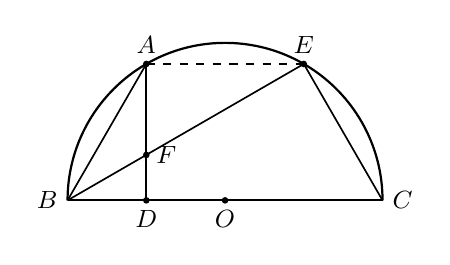
\begin{tikzpicture}[>=stealth, semithick, font=\small, scale=1.0]
  \draw[thick] (-2,0) arc (180:0:2);
  \draw[thick] (-2,0)--(2,0);
  \coordinate (B) at (-2,0); \coordinate (C) at (2,0);
  \coordinate (A) at (-1,1.732); \coordinate (E) at (1,1.732);
  \coordinate (D) at (-1,0); \coordinate (O) at (0,0);
  \coordinate (F) at (-1,0.577);
  \draw (A)--(D); \draw (A)--(B);
  \draw (B)--(E); \draw (E)--(C);
  \draw[dashed] (A)--(E);
  \fill (A) circle (1.2pt) node[above] {$A$};
  \fill (E) circle (1.2pt) node[above] {$E$};
  \fill (F) circle (1.2pt) node[right] {$F$};
  \fill (D) circle (1.2pt) node[below] {$D$};
  \fill (O) circle (1.2pt) node[below] {$O$};
  \node[left] at (B) {$B$};
  \node[right] at (C) {$C$};
\end{tikzpicture}
\end{center}
\nopagebreak[4]
\end{question}
\begin{question}
\gkti{12}设 $S_n$ 是等差数列 $\{a_n\}$（$n\in\mathbf N^*$）的前 $n$ 项和，且 $a_1=1$，$a_4=7$，则 $S_5=$ $\underline{\qquad}$。

\Needspace{0.4\textheight}
\end{question}
\begin{question}
\gkti{13}若执行如图所示的框图，输入 $x_1=1$，$x_2=2$，$x_3=3$，$x=2$，则输出的数等于 $\underline{\qquad}$。
\nopagebreak[4]
\begin{center}% 2011 年湖南卷理科第 13 题：程序框图。
% 来源 PDF：普通高考/2011/2011湖南理.pdf，SHA-256 09b67f1db8e6a280165cf8431211a968163c0d0f262a50068dd607607a9ec578。
% 原页：第 1 页第 3 栏上部，书页码 671。
\begin{tikzpicture}[>=stealth, semithick, font=\small]
  \node[draw, rounded corners=0.12cm, minimum width=1.2cm, minimum height=0.5cm] (start) at (0,0) {开始};
  \node[draw, minimum width=3.2cm, minimum height=0.55cm] (in) at (0,-1.2) {输入 $x_1,x_2,x_3,x$};
  \node[draw, minimum width=2.6cm, minimum height=0.5cm] (init) at (0,-2.4) {$i=1,\ S=0$};
  \node[draw, minimum width=3.2cm, minimum height=0.55cm] (add) at (0,-3.7) {$S=S+(x_i-x)^2$};
  \node[draw, diamond, aspect=1.7, minimum width=1.4cm, minimum height=0.9cm] (test) at (0,-5.1) {$i<3$};
  \node[draw, minimum width=1.6cm, minimum height=0.5cm] (inc) at (2.8,-3.7) {$i=i+1$};
  \node[draw, minimum width=2.2cm, minimum height=0.5cm] (div) at (0,-6.4) {$S=\dfrac1iS$};
  \node[draw, trapezium, trapezium left angle=72, trapezium right angle=108,
        minimum width=1.6cm, minimum height=0.55cm] (out) at (0,-7.6) {输出 $S$};
  \node[draw, rounded corners=0.12cm, minimum width=1.2cm, minimum height=0.5cm] (stop) at (0,-8.7) {结束};
  \draw[->] (start)--(in); \draw[->] (in)--(init); \draw[->] (init)--(add); \draw[->] (add)--(test);
  \draw[->] (test.east) -| (inc.north) node[pos=0.25, above] {是};
  \draw[->] (inc.south) |- (add.east);
  \draw[->] (test.south)--(div.north) node[midway, right] {否};
  \draw[->] (div)--(out); \draw[->] (out)--(stop);
\end{tikzpicture}
\end{center}
\nopagebreak[4]
\end{question}
\begin{question}
\gkti{14}在边长为 $1$ 的正三角形 $ABC$ 中，设 $\overrightarrow{BC}=2\overrightarrow{BD}$，$\overrightarrow{CA}=3\overrightarrow{CE}$，则 $\overrightarrow{AD}\cdot\overrightarrow{BE}=$ $\underline{\qquad}$。

\Needspace{0.4\textheight}
\end{question}
\begin{question}
\gkti{15}如图所示，$EFGH$ 是以 $O$ 为圆心、半径为 $1$ 的圆的内接正方形，将一颗豆子随机地扔到该圆内，用 $A$ 表示事件“豆子落在正方形 $EFGH$ 内”，$B$ 表示事件“豆子落在扇形 $OHE$（阴影部分）内”，则（1）$P(A)=$ $\underline{\qquad}$；（2）$P(B\mid A)=$ $\underline{\qquad}$。
\nopagebreak[4]
\begin{center}% 2011 年湖南卷理科第 15 题：圆内接正方形与扇形 OHE。
% 来源 PDF：普通高考/2011/2011湖南理.pdf，SHA-256 09b67f1db8e6a280165cf8431211a968163c0d0f262a50068dd607607a9ec578。
% 原页：第 1 页第 3 栏中部，书页码 671。
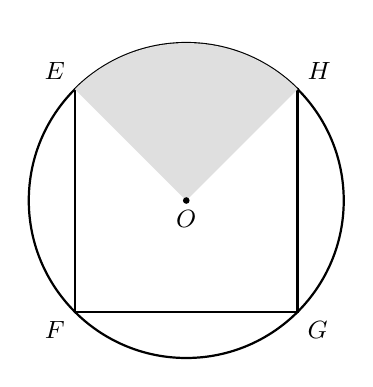
\begin{tikzpicture}[>=stealth, semithick, font=\small, scale=1.0]
  \draw[thick] (0,0) circle (2);
  \coordinate (E) at (-1.414,1.414);
  \coordinate (H) at (1.414,1.414);
  \coordinate (F) at (-1.414,-1.414);
  \coordinate (G) at (1.414,-1.414);
  \draw[thick] (E)--(H)--(G)--(F)--cycle;
  \fill[gray!25] (0,0)--(H) arc (45:135:2)--cycle;
  \fill (0,0) circle (1.2pt) node[below] {$O$};
  \node[above left] at (E) {$E$};
  \node[above right] at (H) {$H$};
  \node[below left] at (F) {$F$};
  \node[below right] at (G) {$G$};
\end{tikzpicture}
\end{center}
\nopagebreak[4]
\end{question}
\begin{question}
\gkti{16}对于 $n\in\mathbf N^*$，将 $n$ 表示为 $n=a_0\times2^k+a_1\times2^{k-1}+a_2\times2^{k-2}+\cdots+a_{k-1}\times2^1+a_k\times2^0$。当 $i=0$ 时，$a_i=1$，当 $1\leqslant i\leqslant k$ 时，$a_i$ 为 $0$ 或 $1$。记 $I(n)$ 为上述表示中 $a_i$ 为 $0$ 的个数（例如：$1=1\times2^0$，$4=1\times2^2+0\times2^1+0\times2^0$，则 $I(1)=0$，$I(4)=2$），则

（1） $I(12)=$ $\underline{\qquad}$；

（2） $\sum\limits_{n=1}^{127}2^{I(n)}=$ $\underline{\qquad}$。

\end{question}
\gkpart{三、解答题}

\begin{question}
\gkti{17}在 $\triangle ABC$ 中，角 $A$，$B$，$C$ 所对的边分别为 $a$，$b$，$c$，且满足 $c\sin A=a\cos C$。

（1） 求角 $C$ 的大小；

（2） 求 $\sqrt3\sin A-\cos\left(B+\dfrac\pi4\right)$ 的最大值，并求取得最大值时角 $A$，$B$ 的大小。

\end{question}
\begin{question}
\gkti{18}某商店试销某种商品 $20$ 天，获得如下数据：

\begin{center}
\begin{tabular}{lllll}
\toprule
日销售量（件） & 0 & 1 & 2 & 3 \\
\midrule
频数 & 1 & 5 & 9 & 5 \\
\bottomrule
\end{tabular}
\end{center}

试销结束后（假设该商品的日销售量的分布规律不变），设某天开始营业时有该商品 $3$ 件，当天营业结束后检查存货，若发现存货少于 $2$ 件，则当天进货补充至 $3$ 件，否则不进货，将频率视为概率。

（1） 求当天商品不进货的概率；

（2） 记 $X$ 为第二天开始营业时该商品的件数，求 $X$ 的分布列和数学期望。

\Needspace{0.4\textheight}
\end{question}
\begin{question}
\gkti{19}如图，在圆锥 $PO$ 中，已知 $PO=\sqrt2$，$\odot O$ 的直径 $AB=2$，$C$ 是 $\overset{\frown}{AB}$ 的中点，$D$ 为 $AC$ 的中点。

（1） 证明：平面 $POD\perp$ 平面 $PAC$；

（2） 求二面角 $B-PA-C$ 的余弦值。
\nopagebreak[4]
\begin{center}% 2011 年湖南卷理科第 19 题：圆锥 PO，C 为半圆 AB 中点，D 为 AC 中点。
% 来源 PDF：普通高考/2011/2011湖南理.pdf，SHA-256 09b67f1db8e6a280165cf8431211a968163c0d0f262a50068dd607607a9ec578。
% 原页：第 2 页第 1 栏下部，书页码 672。示意。
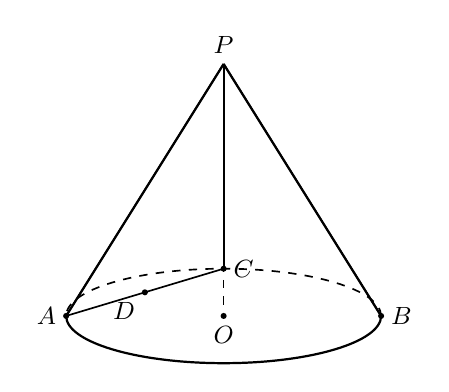
\begin{tikzpicture}[>=stealth, semithick, font=\small, scale=1.0]
  \draw[thick] (0,3.2)--(-2,0);
  \draw[thick] (0,3.2)--(2,0);
  \draw[thick] (-2,0) arc (180:360:2 and 0.6);
  \draw[dashed] (2,0) arc (0:180:2 and 0.6);
  \draw[dashed] (0,3.2)--(0,0);
  \coordinate (A) at (-2,0);
  \coordinate (B) at (2,0);
  \coordinate (C) at (0,0.6);
  \coordinate (D) at (-1,0.3);
  \draw[thick] (0,3.2)--(C);
  \draw (A)--(C);
  \draw (0,3.2)--(A);
  \draw (0,3.2)--(B);
  \fill (A) circle (1.1pt) node[left] {$A$};
  \fill (B) circle (1.1pt) node[right] {$B$};
  \fill (C) circle (1.1pt) node[right] {$C$};
  \fill (D) circle (1.1pt) node[below left] {$D$};
  \fill (0,0) circle (1.1pt) node[below] {$O$};
  \node[above] at (0,3.2) {$P$};
\end{tikzpicture}
\end{center}
\nopagebreak[4]
\Needspace{0.4\textheight}
\end{question}
\begin{question}
\gkti{20}如图，长方体物体 $E$ 在雨中沿面 $P$（面积为 $S$）的垂直方向作匀速移动，速度为 $v$（$v>0$），雨速沿 $E$ 移动方向的分速度为 $c$（$c\in\mathbf R$）。$E$ 移动时单位时间内的淋雨量包括两部分：① $P$ 或 $P$ 的平行面（只有一个面淋雨）的淋雨量，假设其值与 $|v-c|\times S$ 成正比，比例系数为 $\dfrac1{10}$；② 其它面的淋雨量之和，其值为 $\dfrac12$。记 $y$ 为 $E$ 移动过程中的总淋雨量，当移动距离 $d=100$，面积 $S=\dfrac32$ 时。

（1） 写出 $y$ 的表达式；

（2） 设 $0<v\leqslant10$，$0<c\leqslant5$，试根据 $c$ 的不同取值范围，确定移动速度 $v$，使总淋雨量 $y$ 最少。
\nopagebreak[4]
\begin{center}% 2011 年湖南卷理科第 20 题：雨中移动的长方体。
% 来源 PDF：普通高考/2011/2011湖南理.pdf，SHA-256 09b67f1db8e6a280165cf8431211a968163c0d0f262a50068dd607607a9ec578。
% 原页：第 2 页第 2 栏上部，书页码 672。示意。
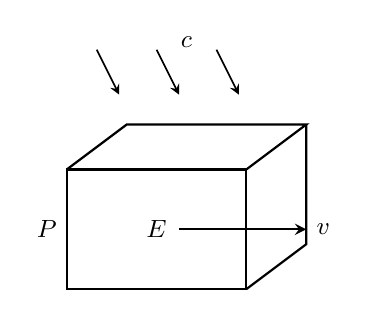
\begin{tikzpicture}[>=stealth, semithick, font=\small, scale=0.95]
  \draw[thick] (0,0)--(2.4,0)--(2.4,1.6)--(0,1.6)--cycle;
  \draw[thick] (0,1.6)--(0.8,2.2)--(3.2,2.2)--(2.4,1.6);
  \draw[thick] (2.4,0)--(3.2,0.6)--(3.2,2.2);
  \node at (1.2,0.8) {$E$};
  \draw[->, thick] (1.5,0.8)--(3.2,0.8) node[right] {$v$};
  \foreach \x in {0.4,1.2,2.0} \draw[->] (\x,3.2)--(\x+0.3,2.6);
  \node at (1.6,3.3) {$c$};
  \node[left] at (0,0.8) {$P$};
\end{tikzpicture}
\end{center}
\nopagebreak[4]
\Needspace{0.4\textheight}
\end{question}
\begin{question}
\gkti{21}如图，椭圆 $C_1:\dfrac{x^2}{a^2}+\dfrac{y^2}{b^2}=1$（$a>b>0$）的离心率为 $\dfrac{\sqrt3}2$，$x$ 轴被曲线 $C_2:y=x^2-b$ 截得的线段长等于 $C_1$ 的长半轴长。

（1） 求 $C_1$，$C_2$ 的方程；

（2） 设 $C_2$ 与 $y$ 轴的交点为 $M$，过坐标原点 $O$ 的直线 $l$ 与 $C_2$ 相交于点 $A$，$B$，直线 $MA$，$MB$ 分别与 $C_1$ 相交于点 $D$，$E$。

① 证明：$MD\perp ME$；

② 记 $\triangle MAB$，$\triangle MDE$ 的面积分别是 $S_1$，$S_2$。问：是否存在直线 $l$，使得 $\dfrac{S_1}{S_2}=\dfrac{17}{32}$？请说明理由。
\nopagebreak[4]
\begin{center}% 2011 年湖南卷理科第 21 题：椭圆 C1 与抛物线 C2。
% 来源 PDF：普通高考/2011/2011湖南理.pdf，SHA-256 09b67f1db8e6a280165cf8431211a968163c0d0f262a50068dd607607a9ec578。
% 原页：第 2 页第 2 栏下部，书页码 672。示意。
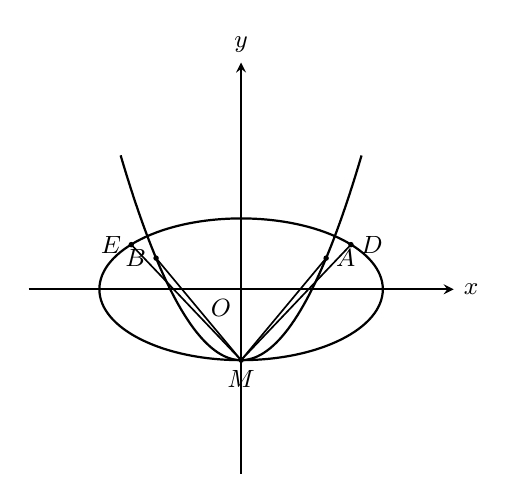
\begin{tikzpicture}[>=stealth, semithick, font=\small, scale=0.9]
  \draw[->] (-3,0)--(3,0) node[right] {$x$};
  \draw[->] (0,-2.6)--(0,3.2) node[above] {$y$};
  \draw[thick] (0,0) ellipse (2 and 1);
  \draw[thick, domain=-1.7:1.7, samples=80] plot (\x,{\x*\x-1});
  \coordinate (M) at (0,-1);
  \coordinate (A) at (1.2,0.44);
  \coordinate (B) at (-1.2,0.44);
  \coordinate (D) at (1.55,0.63);
  \coordinate (E) at (-1.55,0.63);
  \draw (A)--(M)--(B);
  \draw (D)--(M)--(E);
  \fill (M) circle (1.1pt) node[below] {$M$};
  \fill (A) circle (1.1pt) node[right] {$A$};
  \fill (B) circle (1.1pt) node[left] {$B$};
  \fill (D) circle (1.1pt) node[right] {$D$};
  \fill (E) circle (1.1pt) node[left] {$E$};
  \node[below left] at (0,0) {$O$};
\end{tikzpicture}
\end{center}
\nopagebreak[4]
\end{question}
\begin{question}
\gkti{22}已知函数 $f(x)=x^3$，$g(x)=x+\sqrt x$。

（1） 求函数 $h(x)=f(x)-g(x)$ 的零点个数，并说明理由；

（2） 设数列 $\{a_n\}$（$n\in\mathbf N^*$）满足 $a_1=a$（$a>0$），$f(a_{n+1})=g(a_n)$，证明：存在常数 $M$，使得对于任意的 $n\in\mathbf N^*$，都有 $a_n\leqslant M$。

\end{question}